\documentclass[UTF8]{ctexart}

\usepackage[ruled]{algorithm2e}
\usepackage{amsmath}
\usepackage{amssymb}
\usepackage{appendix}
\usepackage{enumerate}
\usepackage{fontspec}
\usepackage{geometry}
\usepackage{graphicx}
\usepackage{setspace}
\usepackage{subfigure}
\usepackage{url}
\usepackage{xeCJK}

\title{实现自适应空间文本分割树}
\author{王梓涵\quad 周昕逸\quad 刘权}
\date{}
\bibliographystyle{plain}

\geometry{left=2.5cm,right=2.5cm,top=2.5cm,bottom=2.5cm} 
\pagestyle{plain}
\setmonofont{Consolas}

\begin{document}
\maketitle

\linespread{0.5}
\setlength{\parskip}{0.5\baselineskip}

\section{理论介绍}

在日常的信息传播中,常常需要处理用户所提供的一系列包含空间和关键词的查询项。例如:一些基于位置信息的推荐系统可根据用户的需求推送相关产品的信息,Twitter等社交网络可分析用户发布的内容及附带的地理位置标签推送他们感兴趣的内容。本文实现的自适应空间文本分割树(Adaptive spatial-textual Partition Tree,以下简称AP树)可以通过自动计算关键词和空间因子两种分割方式的代价选择合适的匹配方式。

AP树的实现有三大挑战。第一,在实际应用中的数据量极大,算法效率的提升可以节省很多成本。第二,算法吞吐量要大以应对源源不断的包含空间文本信息的对象流。第三,需要建立新的空间因子和关键词的索引机制用于不同的分配方法。

AP树的基本运算包含三个部分。匹配对象和查询项的算法,计算关键词和空间因子分割代价的模型和建立索引的算法。

AP树包含三种类型的结点:关键词结点(k-node),空间结点(s-node)和查询项结点(q-node)。一棵AP树的叶子结点都是q-node,每一个查询项都可根据其关键词和空间因子被分配入一个或多个叶子结点中。运用关键词分割方法的结点称为k-node。我们认为所有的关键词都包含于一个有序的词典中,它们的相对位置是确定的,因此可以比较大小。每一层的k-node中包含了其叶子结点对应的查询项的第$l$个关键词的划分(cuts),$l$为结点所在的层次。运用空间面积分割方法的结点称为s-node。每一层的s-node中包含了其叶子结点对应的查询项的面积划分(cells)。如果一个查询项没有足够的关键词,无法寻找到一个对应的cut,就用一个dummy cut保存;如果一个查询项的覆盖面积已经包含一个s-node的覆盖面积,就用一个dummy cell保存。

在匹配对象时,使用深度优先搜索法。如果当前结点是q-node,则判断该对象是否与q-node中的查询项匹配,如果匹配则可等待输出。如果当前结点是s-node,则访问它的cell和dummy cell。如果当前结点是k-node,则访问它的cut和dummy cut。

AP树还提供了一个计算两种分割匹配算法的代价的模型。匹配代价$C(P)$的定义为:
\[C(P)=\sum_{i=1}^f \mathbf{w}(B_i)\times \mathbf{p}(B_i)\]
其中$B$是一种分割方式,$\mathbf{w}(B)$是与$B$有关的查询项的个数,$\mathbf{p}(B)$是$B$的击中概率,即在对象匹配过程中$B$被访问的可能性。在关键词分割法中,$\mathbf{p}(B)=\sum_{w\in B} \mathbf{p}(w)$,其中$\mathbf{p}(w)=\frac{freq(w)}{\sum_{w\in P}freq(w)}$,$freq(w)$为关键词$w$在所有查询项中出现的频率。在空间分割法中$\mathbf{p}(B)=\frac{Area(B)}{Area(N)}$,$Area(B)$是$B$的面积,$Area(N)$是结点$N$的区域面积。接着使用启发式算法寻找使得匹配代价最小的关键词的分割和空间的分割。

AP树还提供了建立索引的方法。使用两个标志$kP$和$sP$来表示所有的查询项是否可以进一步地进行关键词的分割和空间的分割,并通过计算两种分割方式的代价$C_k$和$C_s$确定当前结点使用哪种分割方式。


\section{代码实现}

\subsection{接口设计}
首先定义所涉及的两个结构体:空间文本对象\texttt{STObject}以及查询项\texttt{Query}。\texttt{STObject}有两个成员:\texttt{Pointf}类型的位置\texttt{location}以及\texttt{std::set<std::string>}类型的关键词集合\texttt{keywords}。\texttt{STObject}也有两个成员:\texttt{Boundf}类型的方形区域\texttt{region}和\texttt{std::set<std::string>}类型的关键词集合\texttt{keywords},其中\texttt{Boundf}为由两个\texttt{Pointf}确定的轴对齐包围区域。类的使用者需要通过这两个结构来和类进行交互。

本文所实现的AP树,是一种空间文本分割树,定义抽象的空间文本分割树类\texttt{STTree},其有两个纯虚函数\texttt{std::vector<Query> Match(const STObject \&) const}和\texttt{void Register(const \\std::vector<Query> \&)}。AP树类\texttt{APTree}继承自\texttt{STTree}。\texttt{APTree}的构造函数声明为\texttt{APTree(const std::vector<std::string> \&vocab, const std::vector<Query> \&queries, size\_t f, size\_t theta\_Q, size\_t theta\_KL)},其中\texttt{vocab}为所有的关键词,\texttt{queries}为需要注册的查询项,\texttt{f}、\texttt{theta\_Q}和\texttt{theta\_KL}均为论文中明确给出的参数。

\subsection{存储实现}
由于AP树存储的数据体量大,树的构建和查询算法较为复杂,为了能够发挥AP树的优势,在内部存储方式的实现上需要一定的构思。

首先介绍AP树内部对于空间文本对象和查询项的存储。在\texttt{APTree}内部,使用\texttt{STObjectNested}和\texttt{QueryNested}来分别表示这两种结构。在两种结构中,位置信息,即\texttt{location}和\texttt{region}保持原样,而\texttt{keywords}变为\texttt{std::vector<size\_t>}类型,其中\texttt{std::vector}所存储的是该关键词在关键词词汇\texttt{vocab}中的索引。考虑到字符串的比较较为耗时,而整数的比较效率较高,在建树和查找的过程中可以直接对序号进行操作,而非对字符串。同时,由于AP树算法中有对\texttt{keywords}随机访问的需求,应该将其从原来的\texttt{std::set}转为\texttt{std::vector}以实现高效的随机访问。

然后介绍关键词分割方案和空间分割方案的存储表示。关键词分割方案用\texttt{KeywordPartition}结构体表示,其成员,包括:类型为\texttt{std::unique\_ptr<KeywordCut[]>}分割序列\texttt{cuts},其中\texttt{KeywordCut}为关键词序号的闭区间;类型为\texttt{std::unique\_ptr<std::vector<QueryNested *>[]>}的查询项查找表\texttt{queries},用来表示每个关键词闭区间对应哪些查询项,注意到这里使用的是\texttt{QueryNested}的指针类型,这是为了节约运行时内存占用,避免\texttt{QueryNested}的多次复制;类型为\texttt{std::vector<\\QueryNested *>}的dummy cut表\texttt{dummy};还有一个表示该分割方案代价的浮点数\texttt{cost}。空间分割方案用\texttt{SpatialPartition}结构体表示,其成员包括:类型为\texttt{size\_t},在X、Y轴上个各自的分割数目\texttt{nPartX}、\texttt{nPartY};类型为\texttt{std::unique\_ptr<double[]>}的分割位置\texttt{partX},\texttt{partY};类型为\texttt{std::unique\_ptr<std::vector<QueryNested *>[]>}的单元格查询项序列\texttt{cells},注意这是一个一维的数组,一个二维的单元格索引需要通过运算转为一维的数组索引;剩下的\texttt{dummy}和\texttt{cost}与\texttt{KeywordPartition}相同,不作赘述。

最后介绍AP树的结点类型\texttt{Node},由于AP树有三种结点类型,而每个结点的子节点的类型父节点是不清楚的,这里使用一个\texttt{NodeType}枚举来标记每个子节点的类型。同时每个结点需要存储结点的关键词偏置\texttt{offset}、区域\texttt{bound},以及是否从关键词和空间信息来划分结点\texttt{useKw}、\texttt{useSp}。对于三种结点各自的信息,定义了\texttt{Node}的内部结构体来储存。为了节约结点空间,使用\texttt{std::unique\_ptr}来实现较为灵活的管理,默认状况下为\texttt{nullptr},当结点信息完备时,再根据结点类型动态地分配相应的存储空间。q-node类型\texttt{QueryNode}内只需要存储一个\texttt{std::vector<QueryNested>}即可。k-node类型\texttt{KeywordNode}和s-node类型\texttt{SpatialNode}的成员分别与\texttt{KeywordPartition}和\texttt{SpatialPartition}成员类似,不同之处在于:\texttt{KeywordNode}和\texttt{SpatialNode}内不需要存储\texttt{cost}信息,各自的查找表内存储的是\texttt{std::unique\_ptr<Node>},而非\texttt{QueryNested *}。同时\texttt{KeywordNode}和\texttt{SpatialNode}还存有上次构建时包括的查询项数目\texttt{nOld}和上一次构建后新增的查询项数目\texttt{nAdd},便于重构时计算KL散度。由于k-node和s-node内共有dummy cut,考虑将其放在\texttt{Node}的一个\texttt{std::unique\_ptr}中,避免重复定义。这样一来,\texttt{APTree}析构的时候所有内存空间可以自动回收,不需要手动\texttt{delete},也不会造成内存泄漏。

\subsection{运算实现}
AP树的构建和查询算法基本根据原论文所给的伪代码来实现,以下的介绍只作大致思路的梳理和部分要点的提示。

在构造函数里,首先根据参数\texttt{vocab}将\texttt{Query}转成\texttt{QueryNested},并取址,建立\texttt{std::vector <QueryNode *>},然后从根节点开始调用私有\texttt{build}函数。在\texttt{build}函数内,若当前结点判定为q-node,则将传入的\texttt{std::vector<QueryNode *>}内的指针全部取值储存在\texttt{Node::QueryNode}中;不然则调用私有的\texttt{keywordHeuristic}和\texttt{spatialHeuristic}尝试关键词和空间分割,取代价小的分割方式确定节点类型,将相关信息赋予结点,继续下一层递归。和原论文中算法不同之处在于,$l$、$kP$和$sP$是作为\texttt{Node}的成员来传递的,而非通过函数的实参传递,这是为了便于动态重构。要注意,\texttt{Node}的内存空间要在主调用的\texttt{build}函数内分配,其构造的提示信息\texttt{offset}、\texttt{bound}、\texttt{useKw}和\texttt{useSp}也要在\texttt{Node}构造时赋值;其成员的具体类型,以及每种类型下的数据,要在被调用的\texttt{build}函数内分配和赋值。

下面介绍\texttt{keywordHeuristic}和\texttt{spatialHeuristic}内的实现。由于它们均为启发式算法,有相似的思路。首先,对传入的查询项进行\textbf{统计},关键词分割时分别统计当前offset以及所有offset的词频,空间分割时统计边界位置。然后,对统计的对象进行\textbf{均分},关键词分割时均分关键词到每个cut,空间分割时均分边界到每个cell。接着尝试改变划分的边界,找到局部最优的划分,\textbf{改善}整体的代价。最后,利用找到的最佳划分,将查询项\textbf{分配}到每个cut或者cell内,算法结束。

在\texttt{Match}函数内,首先将\texttt{STObject}转成\texttt{STObjectNested},调用私有的\texttt{match}函数进行匹配,匹配算法完全按照论文中的伪代码实现。将得到的\texttt{std::set}内的\texttt{QueryNested}转成\texttt{Query},返回给类的使用者。

\subsection{查询项维护}

\begin{spacing}{1.0}
\begin{algorithm}[H]
\caption{动态注册查询项}
\LinesNumbered
\KwIn{结点$N$,新增查询项$Q$}
\KwOut{新结点$N'$}
\eIf{$N$为q-node}{
    \eIf{$|N.Q.\psi|+|Q.\psi|<\theta_q$}{
        $N.Q\leftarrow$归并$N.Q$和$Q$ \\
        返回$N$
    }{
        $Q'\leftarrow$归并$N.Q$和$Q$ \\
        构建索引($N'$, $Q'$) \\
        返回$N'$
    }
}{
    统计$Q$的信息 \\
    $D_{KL}\leftarrow$计算KL散度 \\
    \eIf{$D_{KL}>\theta_{KL}$}{
        $Q'\leftarrow$归并$N.Q$和$Q$ \\
        构建索引($N'$, $Q'$) \\
        返回$N'$
    }{
        $Q_D\leftarrow$ 寻找$Q$中的dummy查询项 \\
        \If{$Q_D$非空}{
            \eIf{$N$有dummy cut/cell $N_D$}{
                $N_D'\leftarrow$注册($N_D$, $Q_D$) \\
                重置$N$的dummy结点为$N_D'$
            }{
                构建索引($N_D$, $Q_D$)
            }
        }
        \ForEach{$N$中分割$B_i$}{
            $Q_{B_i}\leftarrow$在$Q$中寻找匹配$B_i$的查询项 \\
            $N_{B_i}'\leftarrow$注册($N_{B_i}$, $Q_{B_i}$) \\
            重置$N_{B_i}$的结点为$N_{B_i}'$
        }
        返回$N$
    }
}
\end{algorithm}
\end{spacing}

\texttt{APTree}还实现了查询项的动态注册。原文中只对其做了简单的介绍,没有进行详细的阐述。本文尝试给出其完整的算法伪代码,并对其中的重点问题进行探讨。由于现有的函数已经能够根据一个结点的初始信息和待构建的查询项构建一棵子树,该算法主要解决的是一个结点要不要重构,以及重构后如何让父结点指向重构后的结点的问题。

首先要回答的是要不要重构的问题。原论文中,作者提到要用分割的KL散度$D_{KL}(\textbf{w}_{old}|\textbf{w})$是否超过阈值$\theta_{KL}$来判断。对于定义在相同概率空间上的离散概率分布$P$和$Q$,它们的KL散度定义为
\[D_{KL}(P|Q)=-\sum_{x\in X} P(x)\mathrm{log}(\frac{Q(x)}{P(x)})\]
在AP树的理论中,对每个结点的分割$B$,则有
\[D_{KL}(\textbf{w}_{old}|\textbf{w})=-\sum_{i=1}^f \textbf{w}_{old}(B_i) \mathrm{log}(\frac{\textbf{w}(B_i)}{\textbf{w}_{old}(B_i)})\]
实际实现中,要对上述公式变形。注意到分割$B_i$的新权值(即查询项数目)为原先的权值和新增权值之和$\textbf{w}(B_i)=\textbf{w}_{old}(B_i)+\textbf{w}_{add}(B_i)$。取上式的绝对值,并将$\textbf{w}(B_i)$的表达式代入,可得 
\[\begin{split}|D_{KL}(\textbf{w}_{old}|\textbf{w})| 
&= \sum_{i=1}^f \textbf{w}_{old}(B_i) \mathrm{log}(\frac{\textbf{w}_{old}(B_i) + \textbf{w}_{add}(B_i)}{\textbf{w}_{old}(B_i)}) \\
&= \sum_{i=1}^f \textbf{w}_{old}(B_i)\mathrm{log}(1 + \frac{\textbf{w}_{add}(B_i)}{\textbf{w}_{old}(B_i)}) \end{split}\] 
在上述公式中,在$\textbf{w}_{old}(B_i)$确定的情况下,如果$\textbf{w}_{add}(B_i)$越大,$|D_{KL}(\textbf{w}_{old}|\textbf{w})|$就会越大,那么该结点就更有可能被重构,这是符合我们计算KL散度的目的的。

目前KL散度的计算还存在一个问题,就是单个结点的KL散度是个有量纲的值,其大小依赖于注册的所有查询项的规模,这样一来在和$\theta_{KL}$的比较过程中会出现问题。举一个简单的例子,某个AP树的结点$N_1$内原本有10000个查询项,均匀分布在四个分割里,之后动态注册了1000个,这1000个同样均匀分配到四个分割里;另一个AP树中的结点$N_2$内原本有1000个查询项,也均匀分布在四个分割里,之后动态注册了100个,同样均匀分配到四个分割。我们希望$\theta_{KL}$这一阈值对于树中的结点,在不同的查询项规模下,对一定新增查询项和原有查询项的比例,有相似的控制作用。假设$\theta_{KL}$为100,可以计算得到$D_{KL,N_1}=413.9$,$D_{KL,N_2}=41.4$,有$D_{KL,N_1} > \theta_{KL} > D_{KL,N_2}$。也就是说$N_1$需要重构,而$N_2$不需要,两者判断的结果不同。这意味着建构不同的AP树,需要不同的$\theta_{KL}$才能得到相同的效果。为了解决这一问题,考虑将$D_{KL}$规范化,即
\[|\widehat{D_{KL}}(\textbf{w}_{old}|\textbf{w})| = \sum_{i=1}^f \frac{\textbf{w}_{old}(B_i)}{M_{old}}\mathrm{log}(1 + \frac{\textbf{w}_{add}(B_i)}{\textbf{w}_{old}(B_i)})\]
其中$M_{old}$为注册当前一批查询项前所有不重复查询项的数目。这样一来,$D_{KL}$转化成了一个无量纲的值,那么用户指定的$\theta_{KL}$也是一个无量纲的值,并且对于任意规模的查询项都有相同的控制作用。

然后解决如何重构后父子结点关联的问题。这里利用动态注册函数能够返回一个新的节点指针来实现:如果节点需要重构,则返回重构和新的结点的指针,否则则返回原子结点的指针。在父结点的注册函数中,如果发现子结点的注册函数返回了和之前子结点不同的指针,则更新新的子结点指针,否则则保持原指针。

在具体实现中,为了节省内存占用,传入注册函数的$Q$实际上是\texttt{const std::vector<QueryNested *> \&},该算法一定能保证存储新的查询项时,这些指针都能顺利取值。原因要从\texttt{Node}和\texttt{QueryNested}的生命周期来找。将\texttt{QueryNested}的指针“落实”为实际的值只有两种途径:一是动态注册函数里将$N.Q$和$Q$归并,二是在构建索引函数里将$Q$存进q-node。根据上述算法,这两个动作均发生在重置结点之前。那么在执行重置子结点之前,可以保证原先的子树保持原样,而新的子树已经建立完毕。这样只要调用\texttt{std::unique\_ptr}里的\texttt{reset}方法,即可将原先的子树完全析构,并指向新的子结点。

\section{性能测试}
\subsection{时间性能}
以下我们对\texttt{APTree}的时间性能进行测试。构建的时间主要通过总体构建时间来反应,匹配的性能主要通过平均匹配时间来反映,所有的匹配时间均是匹配2000次后的均值。在未提及时,各项参数默认为:
\begin{enumerate}[1)]
\item $f=16, \theta_q=10$;
\item 每个查询项中含3个关键词,共5000个;区域的边长为0.1到0.01间的随机数,在$[0, 1)^2$的空间内均匀分布;
\item 每个空间文本对象含有7个关键词,共2000个,位置服从$[0, 1)^2上$的均匀分布;
\item 总词汇量为2000个。
\end{enumerate}

\textbf{查询项数量的影响}\quad 图\ref{construct_nq}描述了总体构建时间和查询项数目的关系,并进行了曲线拟合。该曲线为二次曲线,说明构建树的时间复杂度近似为$O(|Q|^2)$。图\ref{match_nq}则描述了平均匹配时间和查询项数目的关系,当查询项数量从1250上升到20000个时,匹配时间也有所上升,这符合我们直观的认知。但匹配时间总体比较平稳,说明AP树能够应对大体量的查询任务。

\begin{figure}[htbp]
    \centering
    \begin{minipage}[t]{8cm}
        \centering
        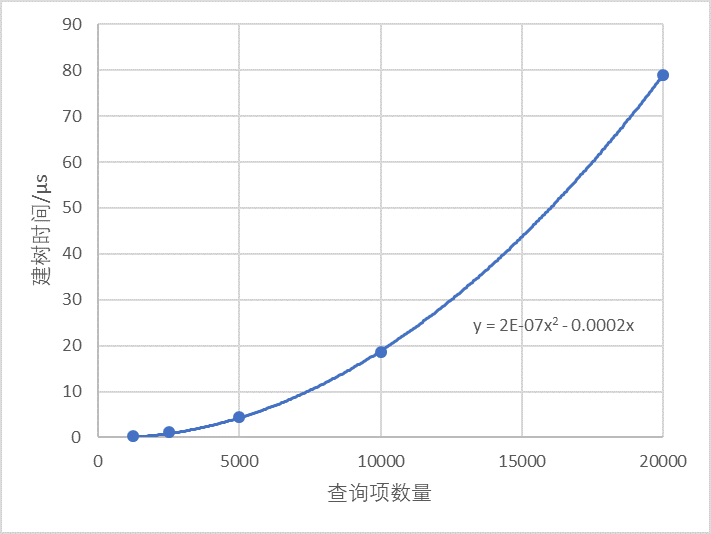
\includegraphics[width=7.5cm]{construct_nq.png}
        \caption{总建树时间与$|Q|$的关系}
        \label{construct_nq}
    \end{minipage}
    \begin{minipage}[t]{8cm}
        \centering
        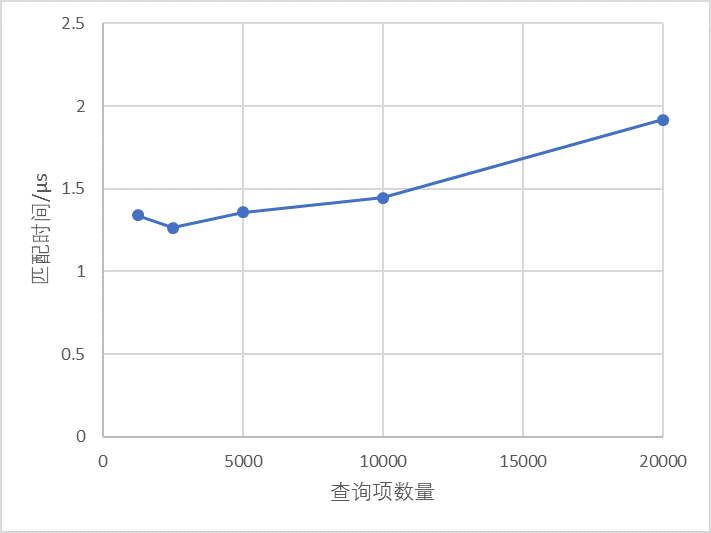
\includegraphics[width=7.5cm]{match_nq.png}
        \caption{平均匹配时间与$|Q|$的关系}
        \label{match_nq}
    \end{minipage}
\end{figure}

\textbf{$f$的影响}\quad 从理论上来说,$f$太小,每个关键词结点的分割数就少,无法完全发挥关键词分割方法的优势。$f$太大,AP树的自适应性就会变差。图\ref{construct_f}描述了建树时间与$f$的关系,图\ref{match_f}描述了匹配时间与$f$的关系。其中$f$的变化范围为10-100。当$f$逐渐增大时,建树时间逐渐增加,匹配时间差异不大。

\begin{figure}[htbp]
    \centering
    \begin{minipage}[t]{8cm}
        \centering
        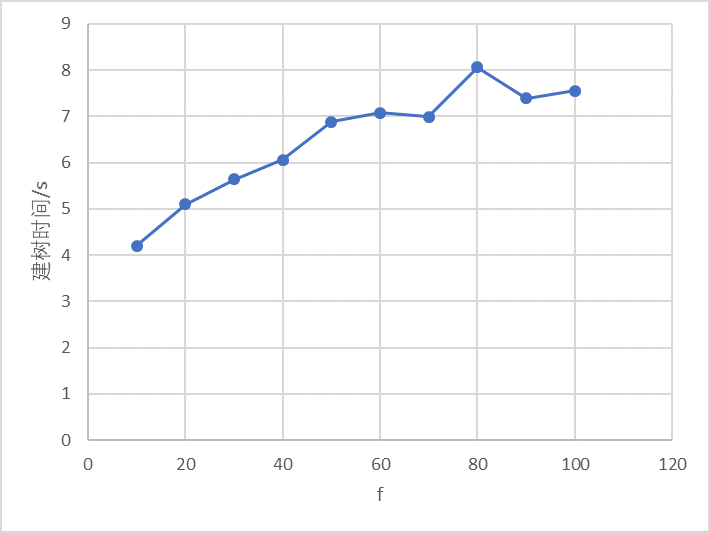
\includegraphics[width=7.5cm]{construct_f.png}
        \caption{总建树时间与$f$的关系}
        \label{construct_f}
    \end{minipage}
    \begin{minipage}[t]{8cm}
        \centering
        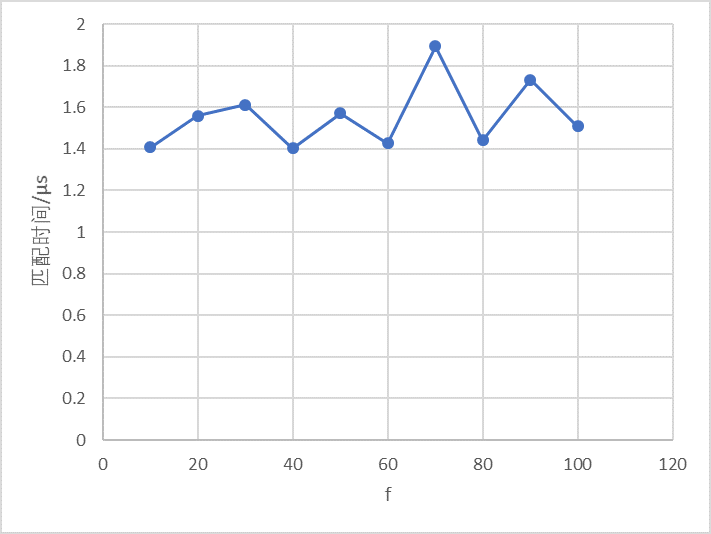
\includegraphics[width=7.5cm]{match_f.png}
        \caption{平均匹配时间与$f$的关系}
        \label{match_f}
    \end{minipage}
\end{figure}

\textbf{$\theta_q$的影响}\quad 图\ref{construct_thetaq}描述了建树时间与$\theta_q$的关系,图\ref{match_thetaq}描述了匹配时间与$\theta_q$的关系。其中$\theta_q$的变化范围为10-100。可以看到$\theta_q$对匹配时间没有什么显著的影响,但对建树时间影响较大。当$\theta_q$小于40时的确起到了限制的作用,导致建树时间变长。当$\theta_q$较大时,实际情况就达不到这个界限了,因此之后的建树时间基本稳定。

\begin{figure}[htbp]
    \centering
    \begin{minipage}[t]{8cm}
        \centering
        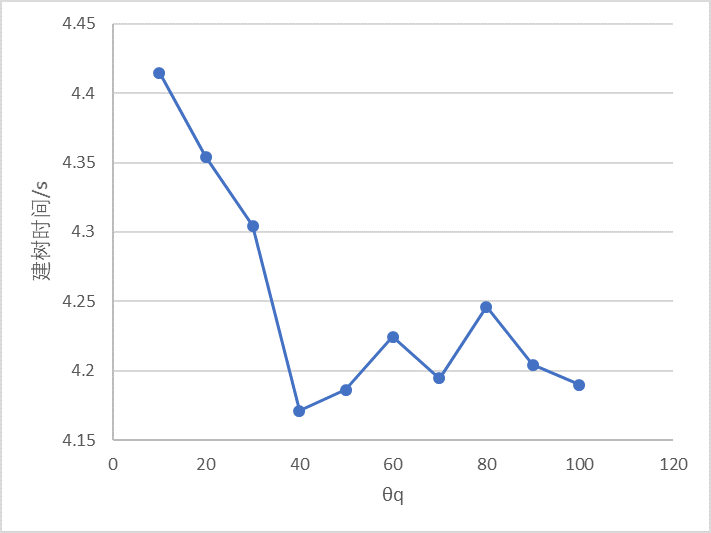
\includegraphics[width=7.5cm]{construct_thetaq.png}
        \caption{总建树时间与$\theta_q$的关系}
        \label{construct_thetaq}
    \end{minipage}
    \begin{minipage}[t]{8cm}
        \centering
        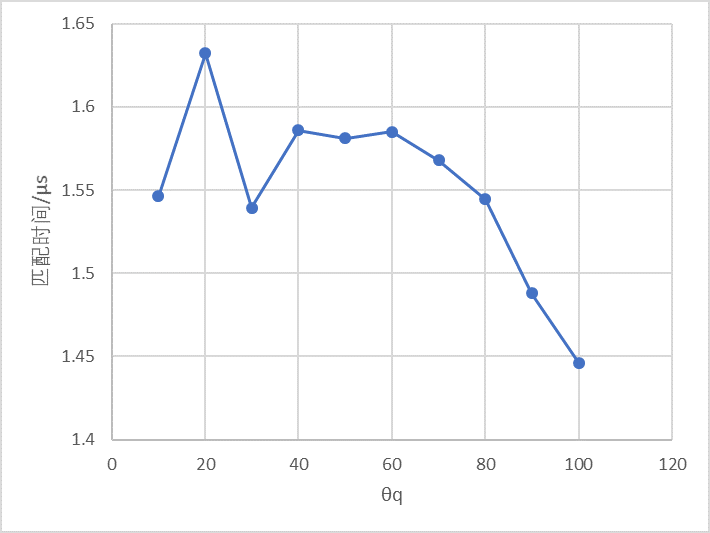
\includegraphics[width=7.5cm]{match_thetaq.png}
        \caption{平均匹配时间与$\theta_q$的关系}
        \label{match_thetaq}
    \end{minipage}
\end{figure}

\textbf{每个查询项中关键词个数的影响}\quad 图\ref{match_nk}描述了关键词个数与匹配时间的关系。由图可知当关键词个数从由2个增加到6个时,匹配时间逐渐下降,因为可能匹配成功的查询项显著减少了,匹配的效率增加了。

\textbf{查询项区域面积的影响}\quad 图\ref{match_reg}描述了查询项区域的面积和匹配时间的关系。为方便实现,通过控制查询项边长的方法控制区域面积的变化。设整个区域面积为1,边长范围为0.00001-0.1。和预想的一样,AP树匹配算法的效率对面积的变化非常敏感。当查询项覆盖面积较大时,其重叠部分增多,导致AP树更可能采用关键词的分割方法。而查询项面积较小时,空间的分割方法优势更大。当边长很小时,查询项的覆盖面积接近于一个点,它落在空间分割的边界上的概率很小,导致空间分割的查找效率变高。

\begin{figure}[htbp]
    \centering
    \begin{minipage}[t]{8cm}
        \centering
        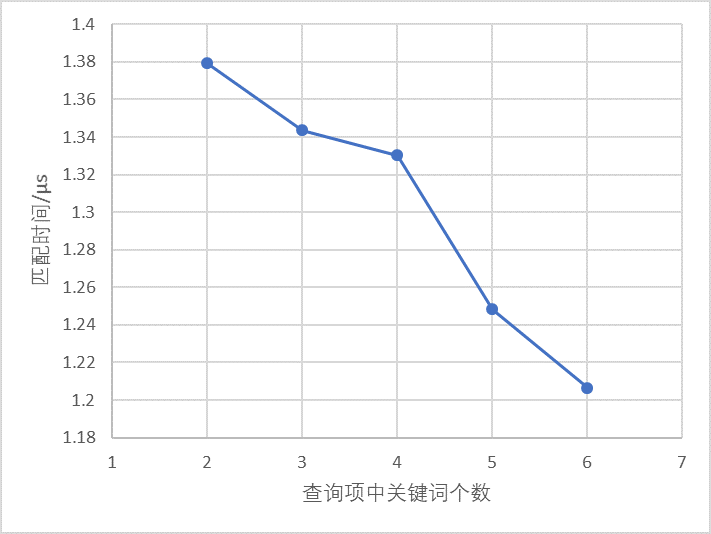
\includegraphics[width=7.5cm]{match_nk.png}
        \caption{平均匹配时间与查询项中关键词个数的关系}
        \label{match_nk}
    \end{minipage}
    \begin{minipage}[t]{8cm}
        \centering
        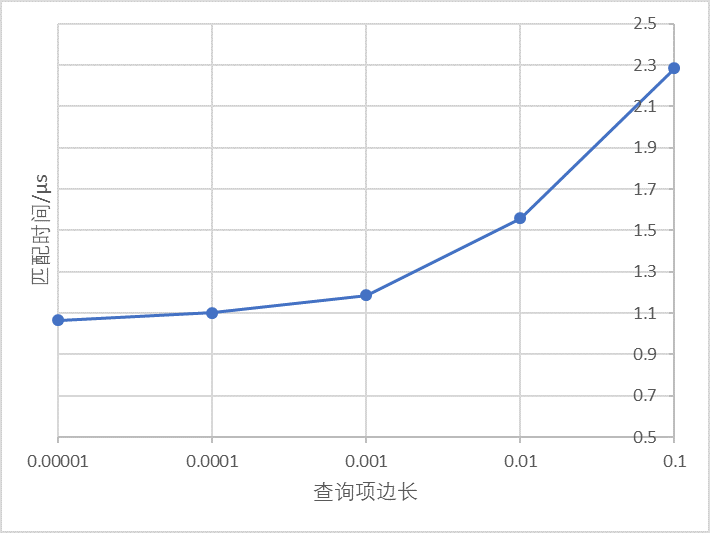
\includegraphics[width=7.5cm]{match_reg.png}
        \caption{平均匹配时间与查询项边长的关系}
        \label{match_reg}
    \end{minipage}
\end{figure}

\subsection{空间性能}
下面我们来考察\texttt{APTree}的空间性能。各项参数和上一节时间性能相同,改变查询项数目,分别测量建树时的峰值内存和建树完毕后稳定的索引内存占用情况。

峰值内存占用如图\ref{ram_peak}所示,可以看到峰值内存占用随查询项个数增长较快,估计空间复杂度在$O(|Q|^{2.2})$左右。这主要是执行启发式算法时,需要存储所有的查询项统计信息所致,而构建根节点时需要统计所有的查询项,所以峰值出现在此时。稳定的索引内存占用如图\ref{ram_stable}所示,可以看到索引内存占用随查询项个数增长较为缓和,估计空间复杂度在$O(|Q|^{1.1})$左右。由于索引内存主要由查询项和结点信息构成,而结点信息与查询项相比少得多,所以空间复杂度只比线性稍微高一点。

\begin{figure}[htbp]
    \centering
    \begin{minipage}[t]{8cm}
        \centering
        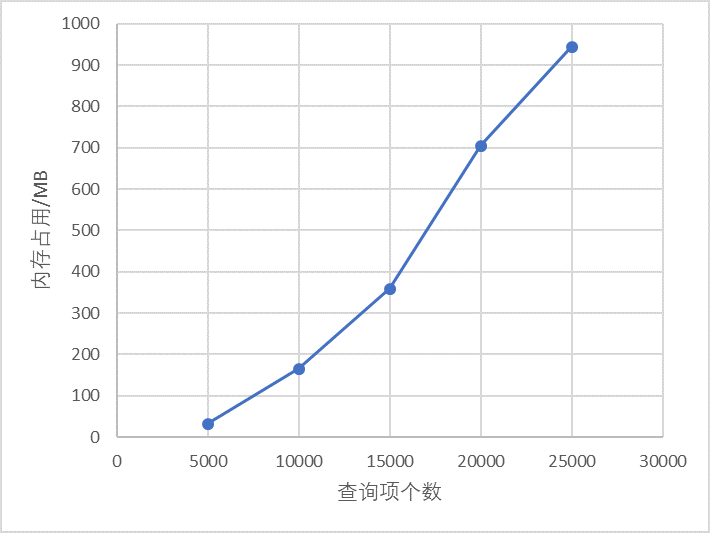
\includegraphics[width=7.5cm]{ram_peak.png}
        \caption{峰值内存与查询项个数的关系}
        \label{ram_peak}
    \end{minipage}
    \begin{minipage}[t]{8cm}
        \centering
        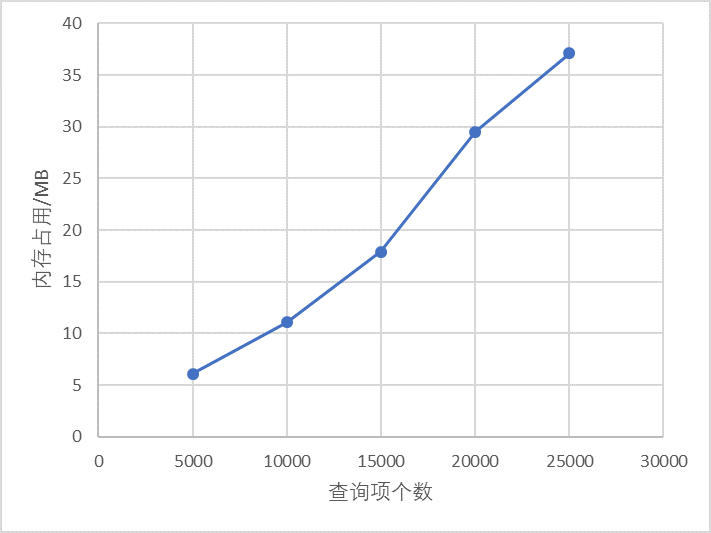
\includegraphics[width=7.5cm]{ram_stable.png}
        \caption{稳定索引内存和查询项个数的关系}
        \label{ram_stable}
    \end{minipage}
\end{figure}

\section{评价}
\subsection{优势}
\begin{enumerate}
    \item AP树在处理不同的数据集时匹配对象的速度快。因为对有些数据集来说关键词和空间两种匹配模式的效率差别很大,AP树可以很好地利用它的自适应性选择最优的匹配方式。
    \item 当AP树应对较多查询项时,依然能保证较高的效率。
    \item AP树可以自动维护它的结构。当工作量发生变化时,它可以根据阈值重构自己的结点,体现出它的自适应性。
\end{enumerate}

\subsection{不足}
\begin{enumerate}
    \item AP树对于空间的需求量较大。在存储实现中可以看到,在树的构建过程中,每一层递归都需要储存对应结点查询项的统计信息。当查询项的总数较大时,势必造成内存占用的激增。在我们的测试中,在注册了10000个查询项后,内存峰值占用就超过了160MB。如果是实际应用中上百万的查询项,其内存占用是相当巨大的。
    \item AP树的构造较为复杂,建树的耗时较长。AP树由于要对两种分割模式进行混合,就要比其它分割树多消耗一倍以上的计算时间。受限于硬件水平,我们的测试中查询项个数仅为5000个,即便如此,AP树的建树时间也已经达到了4s以上,虽然匹配效率较高,但该算法在实际应用中过长的建树时间和维护时间将成为主要的弊端。如果一个数据库系统需要快速地对内部的元素进行迭代、更新,那么AP树显然不适合这样的场景。
\end{enumerate}

\section{未来工作}
由于时间和开发者能力所限,该项目还有许多不完善的地方,在将来可能会对以下方面进行改进或补充。
\begin{enumerate}
    \item 我们的实验中只实现了AP树一种结构,并未实现论文中提到的其他空间文本分割结构,所以无法进行比较,不能体现AP树的优势。今后考虑实现IQ树、$\mathrm{R^t}$树、顺序关键词字典树等结构,进行横向比较。
    \item 当前的\texttt{APTree}尚不具备删除结点的能力,不过在已有函数的基础上可以相对便利地实现这一功能,在今后考虑补充这一功能。
    \item 我们当前的测试只考察了\texttt{APTree}在时间和空间复杂度的性质,对其结点的构造不甚清楚。今后可以考虑设计相应工具,对不同查询项负载和分布下,两种分割方式占比,以及各类结点各自的内存占用等信息,作详尽的分析测试。
\end{enumerate}

\newpage

\begin{appendices}

\section{源代码}
本文所实现的AP树源代码仓库在GitHub上进行托管:\url{https://github.com/wzh99/AP-Tree},采用MIT许可证。

\section{数据集来源}
本文测试所使用的关键词数据集来自US Board on Geographic Names(\url{http://geonames.usgs.gov})

\begin{figure}[htbp]
    \centering
    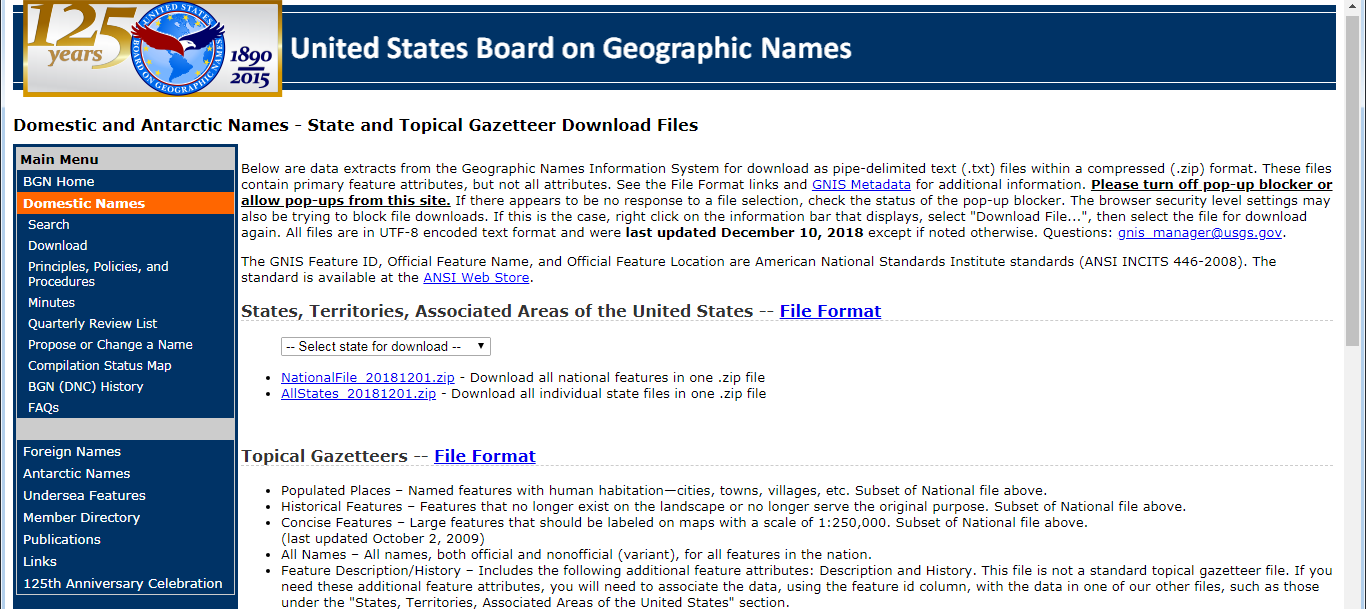
\includegraphics[width=\textwidth]{gn.png}
    \caption{US Board on Geographic Names网站}
\end{figure}

\section{分工}
\begin{itemize}
    \item \textbf{代码实现:} 王梓涵
    \item \textbf{数据测试:} 刘权
    \item \textbf{报告撰写:} 王梓涵\quad 周昕逸\quad 刘权
\end{itemize}

\end{appendices}

\end{document}